% Options for packages loaded elsewhere

\PassOptionsToPackage{unicode}{hyperref}
\PassOptionsToPackage{hyphens}{url}
%
\documentclass[
]{article}
\usepackage{amsmath,amssymb}
\usepackage{iftex}
\ifPDFTeX
  \usepackage[T1]{fontenc}
  \usepackage[utf8]{inputenc}
  \usepackage{textcomp} % provide euro and other symbols
\else % if luatex or xetex
  \usepackage{unicode-math} % this also loads fontspec
  \defaultfontfeatures{Scale=MatchLowercase}
  \defaultfontfeatures[\rmfamily]{Ligatures=TeX,Scale=1}
\fi
\usepackage{lmodern}
\usepackage[a4paper, total={6in, 8in}, top=1in, bottom=2in]{geometry}
\usepackage{xcolor}
\newcommand{\code}[1]{\texttt{#1}}
\definecolor{lightblue}{rgb}{0.8, 0.9, 1} % A light blue color
\newsavebox{\mybox}
\newenvironment{codeblock}{
  \begin{lrbox}{\mybox}\begin{minipage}{\dimexpr\columnwidth-2\fboxsep}
  \ttfamily
}{
  \end{minipage}\end{lrbox}\fcolorbox{black}{lightblue}{\usebox{\mybox}}
}
\ifPDFTeX\else
  % xetex/luatex font selection
\fi
% Use upquote if available, for straight quotes in verbatim environments
\IfFileExists{upquote.sty}{\usepackage{upquote}}{}
\IfFileExists{microtype.sty}{% use microtype if available
  \usepackage[]{microtype}
  \UseMicrotypeSet[protrusion]{basicmath} % disable protrusion for tt fonts
}{}
\makeatletter
\@ifundefined{KOMAClassName}{% if non-KOMA class
  \IfFileExists{parskip.sty}{%
    \usepackage{parskip}
  }{% else
    \setlength{\parindent}{0pt}
    \setlength{\parskip}{6pt plus 2pt minus 1pt}}
}{% if KOMA class
  \KOMAoptions{parskip=half}}
\makeatother
\usepackage{xcolor}
\usepackage{graphicx}
\makeatletter
\def\maxwidth{\ifdim\Gin@nat@width>\linewidth\linewidth\else\Gin@nat@width\fi}
\def\maxheight{\ifdim\Gin@nat@height>\textheight\textheight\else\Gin@nat@height\fi}
\makeatother
% Scale images if necessary, so that they will not overflow the page
% margins by default, and it is still possible to overwrite the defaults
% using explicit options in \includegraphics[width, height, ...]{}
\setkeys{Gin}{width=\maxwidth,height=\maxheight,keepaspectratio}
% Set default figure placement to htbp
\makeatletter
\def\fps@figure{htbp}
\makeatother
\setlength{\emergencystretch}{3em} % prevent overfull lines
\providecommand{\tightlist}{%
  \setlength{\itemsep}{0pt}\setlength{\parskip}{0pt}}
\setcounter{secnumdepth}{-\maxdimen} % remove section numbering
\ifLuaTeX
  \usepackage{selnolig}  % disable illegal ligatures
\fi
\usepackage{bookmark}
\IfFileExists{xurl.sty}{\usepackage{xurl}}{} % add URL line breaks if available
\urlstyle{same}
\hypersetup{
  hidelinks,
  pdfcreator={LaTeX via pandoc}}

\author{}
\date{}

\begin{document}

\begin{center}
\section{Rift HyperBridge: Enabling Trustless Swaps Between Bitcoin and Ethereum}
\end{center}
\vspace*{\baselineskip}

\begin{center}
{Clifford Syner, Tristan Barrett, Samee Siddiqui}
\end{center}

\vspace*{\baselineskip}
\vspace*{\baselineskip}

\begin{center}
\textbf{ABSTRACT}
\end{center}
\

\begin{quote}
\hspace{3em}{We propose Rift, a protocol that enables trustless cross-chain swaps
between Bitcoin and Ethereum by programmatically unlocking escrowed ETH
to a Buyer upon verification of a zero-knowledge proof that the Seller
was paid a specified amount of BTC.}
\end{quote}

\vspace*{\baselineskip}
\vspace*{\baselineskip}


\begin{center}
\textbf{1. INTRODUCTION}
\end{center}
\

\hspace{3em}{Bitcoin and Ethereum are the two largest blockchains in the world by
market cap, yet there is no way to swap between the two assets without
trusting highly centralized intermediaries. Bitcoin holders who want to
enter Ethereum's vibrant dApp ecosystem , and Ethereum users who want to
hold the most widely adopted digital store of value, have no secure way
of doing so. As a result, the liquidity between the two largest
cryptocurrencies remains highly fragmented.}

\hspace{3em}{Trustless cross-chain swaps have been achieved between EVM chains
{[}1{]}, but}{~swaps between Bitcoin and Ethereum are much more complex
due to Bitcoin's lack of smart contracts (making it impossible to verify
the state of Ethereum, escrow funds on-chain, or verify zero-knowledge
proofs)}{, and the prohibitively high gas cost of verifying the state of
Bitcoin on Ethereum using a standard light client.}

\vspace*{\baselineskip}


\hspace{3em}{Users who want to swap between Bitcoin and Ethereum today have 4
options:}

{}

{
\addtolength{\leftmargini}{1cm} % Adjust the 1cm to increase or decrease the indentation
\begin{enumerate}
\tightlist
\item
  {Centralized Exchanges (CEXs)}
\item
  {Institutional Market Makers (OTC Desks)}
\item
  {Collateralized Bitcoin Stablecoins (BTC Stablecoins)}
\item
  {Alternative Layer-1 Blockchains (Alt-L1s)}
\end{enumerate}
}


\vspace*{\baselineskip}


\hspace{3em}{All of these suffer from the same core problems: they are far less
secure than the base chains users hold assets on, and come with other
inherent risks:}
\vspace*{\baselineskip}

\noindent
\hangindent=4.5em
\hangafter=1
\hspace{3em}\textbf{1.} \textbf{Centralized Exchanges}{~}{-}{~}{(e.g. Binance, Coinbase,
ChangeNow, etc.) are controlled by single entities and have historically
struggled to manage user funds, resulting in multiple bankruptcies and
financial losses (e.g. FTX {[}2{]}, Celsius {[}3{]}, etc). CEXs are also
highly regulated, force KYC, rate-limit swapping, and can freeze
customer funds at will.}

\
\noindent
\hangindent=4.5em
\hangafter=1
\hspace{3em}\textbf{2.} \textbf{Institutional Market Makers}{~}{-}{~}{(e.g., Coinbase Custody,
Anchorage Digital, Wintermute, FalconX, Caladan, BitGo, etc.) operate
effectively like CEXs for higher trade sizes. They are fully centralized
and inherit the same security risks as CEXs as a result.}

{}
\noindent
\hangindent=4.5em
\hangafter=1
\hspace{3em}\textbf{3.} \textbf{Collateralized Bitcoin Stablecoins}{~- (e.g. wBTC {[}4{]}, tBTC
{[}5{]}, renBTC, etc.) are a useful primitive but custody Bitcoin in a
high-risk N-of-M multisig wallet where if N keys are compromised, all
collateral can be stolen {[}6{]}. Additionally, since the multisig
ownership is often centralized, they inherit the same censorship and
regulatory risks as CEXs. This has already resulted in the collapse of
renBTC, which once held \textgreater\$1b in collateral {[}7{]}.}

{}
\noindent
\hangindent=4.5em
\hangafter=1
\hspace{3em}\textbf{4.} \textbf{Alt-L1s}{~- (e.g. THORchain {[}8{]}, NEAR Chain Abstraction
{[}9{]}, etc.) are more secure than a multisig, but are far less
decentralized than Bitcoin and Ethereum {[}10, 11, 12{]}, and have far
less capital staked {[}13{]} in the network, leading to much lower
security, uptime, and swapping limits for users. }

{}\vspace*{\baselineskip}


\hspace{3em}{With security via self-custody and decentralization as the core ethos
of blockchain technology, and the increasing demand for swaps between
Bitcoin and Ethereum {[}14{]}, the need for a trustless swapping
protocol between the two largest cryptocurrencies is more apparent than
ever.}

{}\vspace*{\baselineskip}


{}

{}
\begin{center}
\textbf{2. SOLUTION}
\end{center}
{}\vspace*{\baselineskip}


{}

\hspace{3em}{Rift implements a set of zero knowledge circuits }{that verifies a
Buyer paid an arbitrary number of Liquidity Providers (LPs}{) were paid
on Bitcoin, and an on-chain order book smart contract on Ethereum
{[}15{]} that allows Buyers to redeem escrowed ETH deposited by an LP
upon verifying a zk-proof {[}16{]} that the LP(s) were paid in Bitcoin.}

{}

\hspace{3em}{The order book and escrow functionality are combined in a single
``Exchange'' smart contract, which allows anyone to become an LP by
depositing ETH to create a sell order. A sell order specifies an
exchange rate (how much BTC should be paid to unlock the ETH being
deposited) and the LP's Bitcoin payout address. Any Buyer can signal
their intent to fill an order by paying a fee to reserve an LP, locking
that sell order for 8 hours. The Buyer must send the correct amount of
BTC to the reserved LP(s) within this time period, or their reservation
will expire. Once the Buyer sends the agreed-upon amount of Bitcoin to
the reserved LP(s), anyone (including the Buyer) can generate and submit
a zk-proof of this payment by providing the proposed Bitcoin transaction
and associated block data.}

{}
{}\vspace*{\baselineskip}

{Rift verifies 5 invariants before the Buyer can unlock the LPs ETH:}
{}\vspace*{\baselineskip}

{}
\addtolength{\leftmargini}{0.6cm} % Adjust the 1cm to increase or decrease the indentation
\begin{enumerate}
\tightlist
\item
  \code{The proposed block is a valid and safe Bitcoin block. This is done by
  verifying Bitcoin's Proof-of-Work (PoW) {[}17{]} ~consensus mechanism
  and that the proposed block has 6 confirmation blocks built on top of
  it in a ZK circuit.}
\item
  \code{The proposed block contains the multi-output transaction from the
  Buyer to the reserved LP(s). This is done by verifying a Merkle
  inclusion proof {[}18{]} in a ZK circuit.}
\item
  \code{The proposed transaction hash matches the transaction hash in the
  proposed block. This is done by verifying the hash of the transaction
  blob in a ZK circuit.}
\item
  \code{The proposed LP reservation hash matches the hashed reservation data
  in the Exchange contract. This is done by verifying the hash of the
  reservation data in a ZK circuit.}
\item
  \code{The LPs were paid the correct amount of BTC. This is done by
  verifying the UTXO outputs of the Buyer's transaction and that each
  LP receives the BTC amount associated with the SwapReservation in a
  ZK circuit.}
\end{enumerate}

{}
{}\vspace*{\baselineskip}


\hspace{3em}{Once a payment proof is verified, the hash of the block containing the
transaction is stored in a smart contract to be used as a circuit input
for future payment verifications. By implementing a Bitcoin ZK light client, we can verify the state of
Bitcoin on Ethereum while ensuring the same security guarantee as the
Bitcoin network itself (based on computational hashing power). This
allows us to execute arbitrary actions on Ethereum based on verified
changes in Bitcoin's state, thus enabling trustless swaps between the
networks.}

{}\vspace*{\baselineskip}

\begin{center}
\textbf{3. SWAP FLOW}
\end{center}
{}\vspace*{\baselineskip}

{~ ~ ~ ~ ~1. Liquidity Providers (LPs) create sell orders by depositing ETH into
  the Rift Exchange Contract (REC), specifying an exchange rate, and providing a Bitcoin payout
address.}



{}
{}\vspace*{\baselineskip}
\begin{center}
{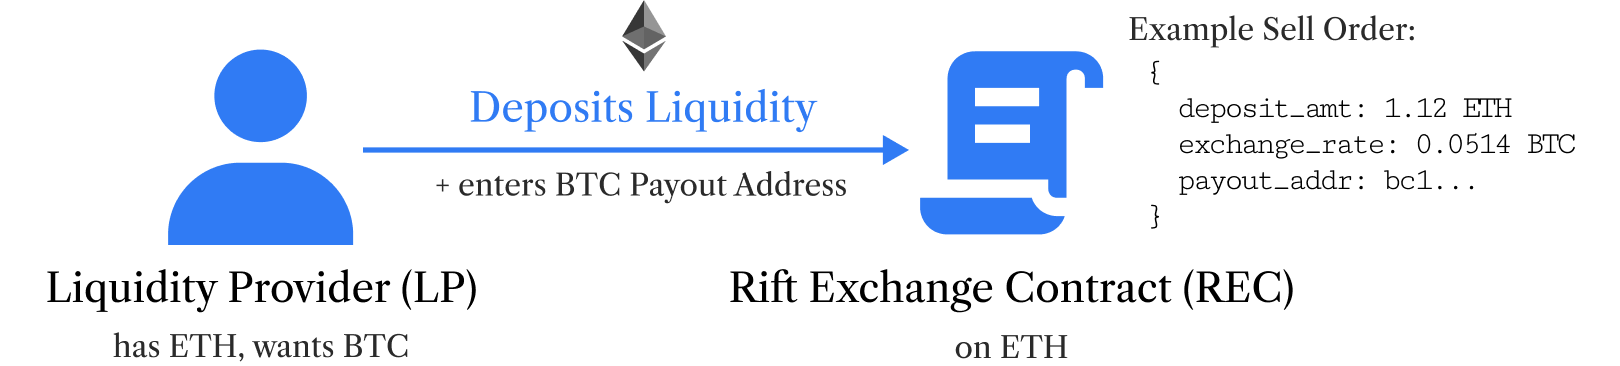
\includegraphics{images/image5.png}}
\end{center}
{}\vspace*{\baselineskip}

{}

{}

{~ ~ ~ ~ ~2. A Bitcoin owner (the Buyer) reserves one or more LPs on the REC and
  pre-pays swap fees in preparation for a swap. This prevents other buyers from attempting to
fill the same order and locks the LP liquidity to prevent mid-swap
withdrawals.}

{}

{}
{}\vspace*{\baselineskip}
\begin{center}
\hspace*{2.8em}{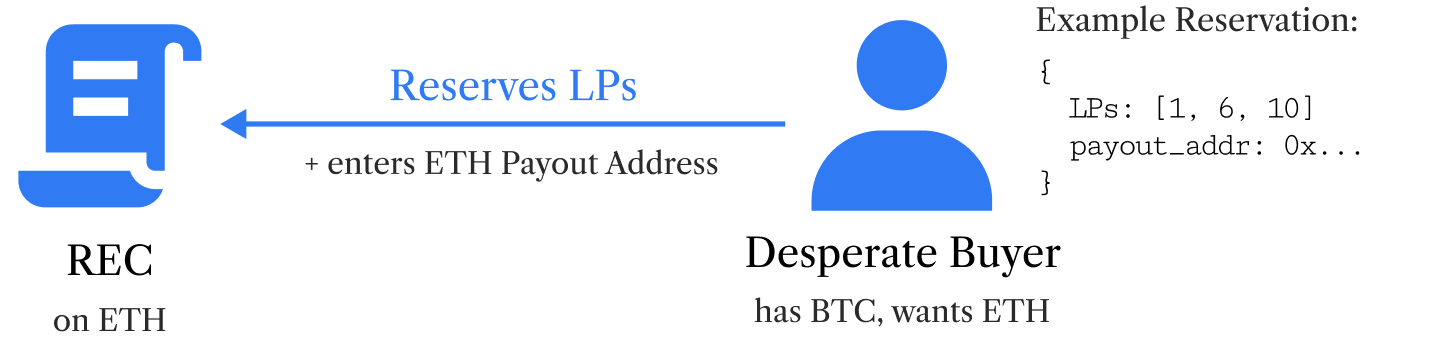
\includegraphics{images/image3.png}}
\end{center}
{}\vspace*{\baselineskip}

{}

{}

{~ ~ ~ ~ ~3. Once LP(s) are reserved the Buyer sends the requested amount of BTC
  to each of the reserved LP(s) in a multi-output transaction with exactly 1 input transaction. The LP
reservation data, along with a unique order nonce is inscribed as part
of the transaction. If an LP is not paid within 8 hours, that LP becomes
unlocked and available for other buyers to reserve.}


{}

{}
{}\vspace*{\baselineskip}
\begin{center}
{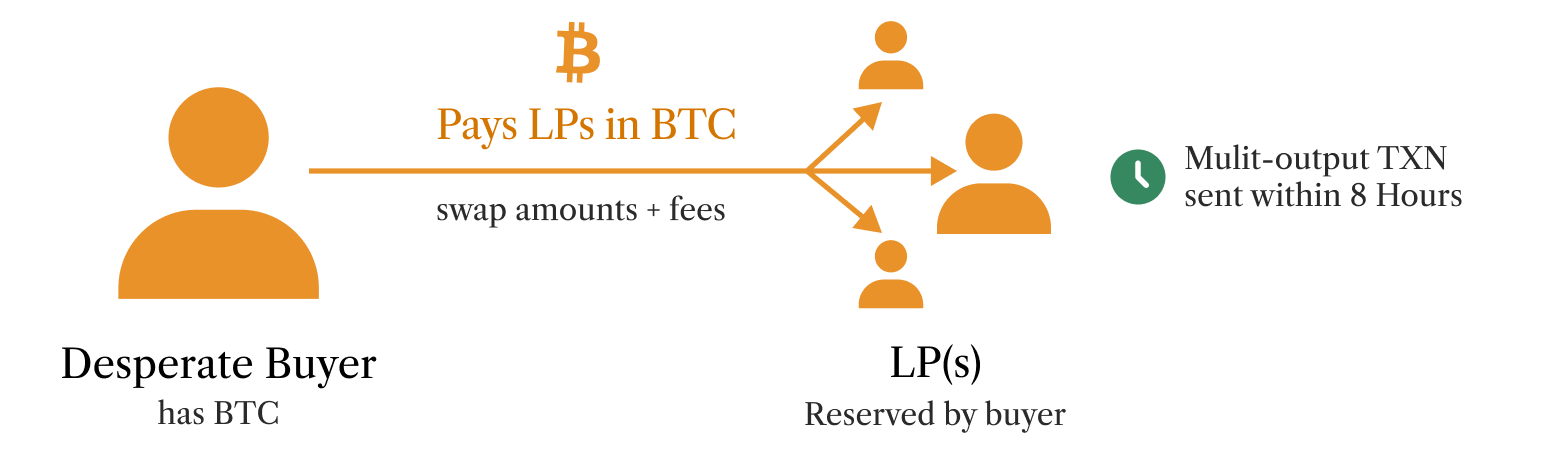
\includegraphics{images/image1.png}}
\end{center}
{}\vspace*{\baselineskip}

{}

{}


{~ ~ ~ ~ ~4. Once the Bitcoin transaction is confirmed, and 6 or more confirmation
  blocks have been built on top of the proposed block, a zk-proof of the payment can be generated
off-chain by anyone and submitted to the REC for verification.}


{}

{}

{}
{}\vspace*{\baselineskip}

{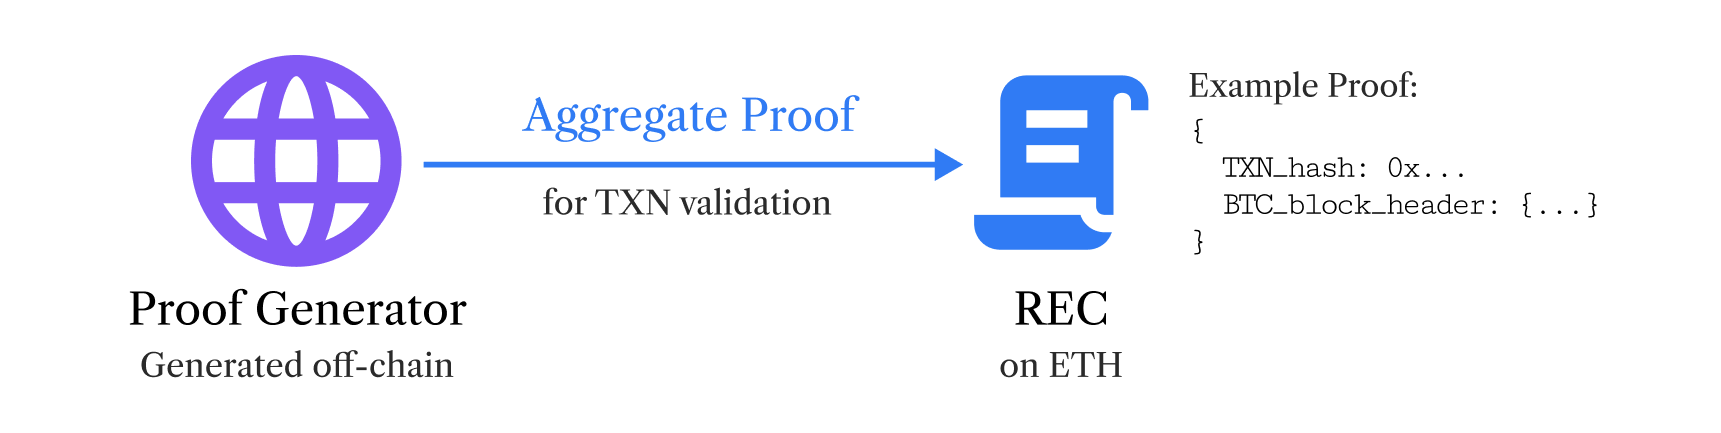
\includegraphics{images/image6.png}}
{}\vspace*{\baselineskip}

{}

{}


{~ ~ ~ ~ ~5. The proposed proof is then passed to the Exchange Verification
  Circuit (EVC), which either verifies or rejects it. Upon verification, a reward and gas rebate is paid out
to the prover.}

{}

{}
{}\vspace*{\baselineskip}

\hspace*{3em}{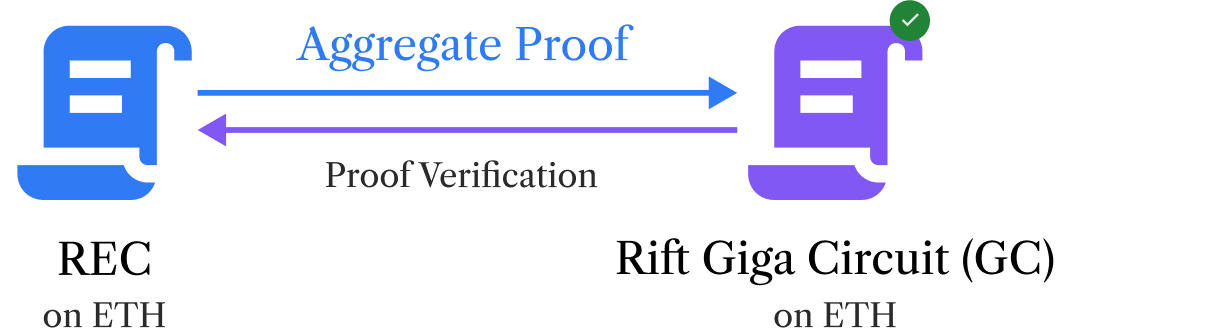
\includegraphics{images/image4.png}}
{}\vspace*{\baselineskip}

{}

{}

{~ ~ ~ ~ ~6. After proof verification and a 10-minute challenge
period, the escrowed ETH can be released (by anyone) to the Buyer's
Ethereum payout address. Upon escrow release, a reward and gas rebate is
paid out to the releaser}{~and the swap is complete.}

{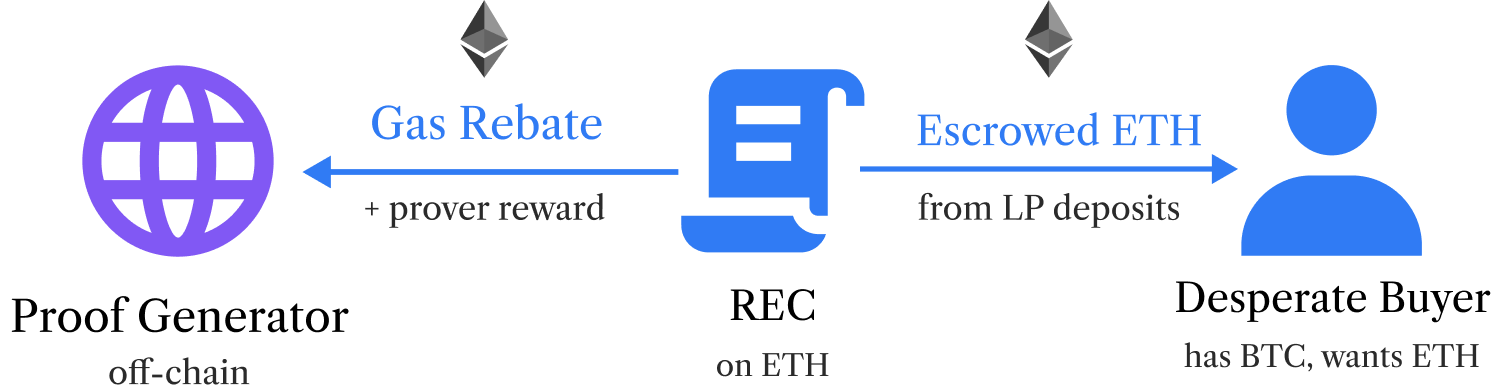
\includegraphics{images/image2.png}}
{}\vspace*{\baselineskip}


\begin{center}
\textbf{4. PROTOCOL}
\end{center}
{}\vspace*{\baselineskip}
{}

\hspace*{3em}{The protocol consists of 2 smart contracts and 5 zk-circuits. The
main components and their functionality are outlined below:}

{}

\hspace*{3em}{Smart Contracts:}

{}
\addtolength{\leftmargini}{0.6cm} % Adjust the 1cm to increase or decrease the indentation
\begin{enumerate}
\tightlist
\item \code{Rift Exchange Contract (REC)}
\item \code{Block Hash Storage Contract (BHSC)}
\end{enumerate}

{}

\hspace*{3em}{Zero-Knowledge Circuits:}

{}

\begin{enumerate}
\tightlist
\item \code  {Rift Giga Circuit (GC)}
\item \code  {Block Verification Circuit (BVC) }
\item \code  {TXN Hash Verification Circuit (TVC)}
\item \code  {LP Hash Verification Circuit (LPVC)}
\item \code  {LP Payment Verification Circuit (PVC)}
\end{enumerate}


{}\vspace*{\baselineskip}

\begin{center}
\textbf{4.1 RIFT EXCHANGE CONTRACT}
\end{center}
{}\vspace*{\baselineskip}
{}

\hspace*{3em}{The REC's purpose is to manage the core exchange logic. The main
components of this are the current order book state, escrow
functionality, and proof verification. These are implemented in 5
primary functions:}

{}

\begin{enumerate}
\tightlist
\item \code{depositLiquidity}
\item \code{withdrawLiquidity}
\item \code{reserveLiquidity}
\item \code{proposeTransactionProof}
\item \code{releaseLiquidity}
\end{enumerate}

{}{}\vspace*{\baselineskip}


\hspace*{3em}\code{depositLiquidity}{~}{is the entry point for LPs to create sell orders.
They deposit ETH, specify an exchange rate, and provide a Bitcoin
address for Buyers to pay them. This creates a
new}{~}{DepositVault:}

\begin{codeblock}

{struct}{~}{DepositVault}{~\{}

\hspace*{3em}{uint256 }{initialBalance}{~}{- }{their deposit amount in ETH}

\hspace*{3em}{uint256 }{unreservedBalance}{~}{- }{the amount available to reserve
from this vault}

\hspace*{3em}{uint64 }{btcExchangeRate}{~}{- }{amount of BTC per 1 ETH, in satoshis}

\hspace*{3em}{bytes32 }{btcPayoutLockingScript }{- }{locking script representing LPs
\hspace*{3em}payout address}

{\}}
\end{codeblock}


{}

\hspace*{3em}{LPs can update the exchange rate on their }\code{DepositVault}{~for any unreserved
liquidity. }\code{withdrawLiquidity}{~allows LPs to cancel their sell order and withdraw
the remainder of their liquidity. This is only possible when liquidity
is not reserved. }\code{reserveLiquidity}{~}{allows Buyers to signal their intent to purchase
by locking one or more }{DepositVaults}{. This prevents two Buyers from
paying the same LP, and guarantees their exchange rate and liquidity
until the swap is completed. }

\hspace*{3em}\code{DepositVaults }{support partial
reservations to maximize the efficiency of liquidity for LPs as well as
available liquidity for Buyers. A Buyer has 8 hours to pay the LPs until
the reservation expires, at which point it becomes available for anyone
to reserve. During this reservation window, LPs cannot withdraw
their reserved capital. To discourage adversarial locking of
liquidity, reservations require paying a percentage of your swap amount
as an upfront fee. Upon successful reservation,
a}{~}\code{SwapReservation}{~is created.}
{}{}\vspace*{\baselineskip}

\begin{codeblock}
{struct}{~}{SwapReservation}{~\{}

\hangindent=19.5em
\hangafter=1
\hspace*{3em}{uint32}{~}{confirmationBlockHeight}{~-}{ The height of the block that confirmed the transaction for this swap.}

\hangindent=18em
\hangafter=1
\hspace*{3em}{uint32}{~}{reservationTimestamp}{~- }{The timestamp when the liquidity reservation was made.}

\hangindent=15.6em
\hangafter=1
\hspace*{3em}{uint32}{~}{unlockTimestamp}{~-}{ The timestamp when the reserved liquidity was unlocked.}

\hangindent=15.5em
\hangafter=1
\hspace*{3em}{ReservationState}{~}{state}{~-}{ The current state of the reservation (unlocked, completed, expired, etc.)}

\hangindent=16.5em
\hangafter=1
\hspace*{3em}{address}{~}{ethPayoutAddress}{~-}{ The Ethereum address where the escrowed ETH will be sent upon successful swap.}

\hangindent=17.5em
\hangafter=1
\hspace*{3em}{bytes32}{~}{lpReservationHash}{~- }{ A hash representing the specific details of the reserved liquidity provider(s).}

\hangindent=19.5em
\hangafter=1
\hspace*{3em}{bytes32}{~}{nonce}{~- }{ A unique identifier used to prevent replay attacks.}

\hangindent=16em
\hangafter=1
\hspace*{3em}{uint256}{~}{totalSwapAmount}{~-}{ The total amount of ETH being swapped in the transaction.}

\hangindent=16.6em
\hangafter=1
\hspace*{3em}{int256}{~}{prepaidFeeAmount}{~-}{~}{ The amount of fees paid upfront when making the reservation.}

\hangindent=15.6em
\hangafter=1
\hspace*{3em}{uint256{[}{]}}{~}{vaultIndexes}{~-}{ Indices of the vaults from which liquidity is reserved.}

\hangindent=17.5em
\hangafter=1
\hspace*{3em}{uint256{[}{]}}{~}{amountsToReserve}{~-}{ Amounts of liquidity reserved from each corresponding vault index.}

{\}}

\end{codeblock}

{}{}\vspace*{\baselineskip}

\hspace*{3em}\code{proposeTransactionProof }{is responsible for verifying the Giga Circuit
proof and updating the \code{Block Hash Storage Contract (BHSC)} with the new block
hashes. Proof verification happens by calling the associated verifier
contract of the \code{Giga Circuit}. Anyone with access to Bitcoin block data
can generate this proof, including the Buyer. If any of the invariants
of the ZK light client return false, it means there was not a valid
payment from the Buyer to the LPs, and proof will be rejected. Upon
successful verification, the pre-paid prover reward is released.}

{}

\hspace*{3em}\code{releaseLiquidity }{releases the escrowed ETH to Buyer's ETH payout
address, along with the pre-paid fee to the releaser, after a 10 minute
challenge period.}{~This will fail }{if a longer chain is proposed
during the challenge period.}

{}{}\vspace*{\baselineskip}
{}\vspace*{\baselineskip}

{}
\begin{center}
\textbf{4.2 BLOCK HASH STORAGE CONTRACT}
\end{center}

{}{}\vspace*{\baselineskip}


\hspace*{3em}{The }{BHSC's}{~purpose is to store the source of truth about which Bitcoin
block hashes are valid, and can be used as inputs for the zk-circuits. Proposed blocks that are verified in the \code{Block Verification Circuit} (Section 4.4) are stored in the BHSC to be used as inputs to verify further proposed blocks building on top of a verified safe block to form the longest chain. Blocks verified by the \code{BVC} are stored using the \code{addBlock} function, called by the \code{REC} to store the verified block height and hash to a mapping in the contract.}
{~}
{}\vspace*{\baselineskip}


\begin{codeblock}
{mapping}{(uint256 =\textgreater{} bytes32) }{blockchain; // block height => block hash}
\\
\\
\
{uint256 public currentHeight;}
\end{codeblock}
\vspace*{\baselineskip}

\hspace*{3em}{The next time }\code{proposeTransactionProof }{from the \code{REC} is called, it
uses the block hash at the previous safe block height as an input into the \code{GC}. If
there is a longer valid chain starting from any previous safe block the mapping is updated with the hashes of
the longer chain and any shorter chain is overwritten. }\code{addBlock }{supports block fast forwarding for up to 24 blocks at a time, so even if there are many Bitcoin blocks between the last swap, the storage contract can be updated with a single verification. In the case of high inactivity and the storage contract falling more than 24 blocks behind Bitcoin, }\code{proposeTransactionProof }{can be called with just block data (no transactions) multiple times until the storage contract is up to date. Since the \code{GC} requires reading inputs from the \code{BSC} to generate a proof, an initial block hash and height must be set by the deployer, but can be easily be verified.}

{}
\vspace*{\baselineskip}
\begin{center}
\textbf{4.3 RIFT GIGA CIRCUIT}
\end{center}

\vspace*{\baselineskip}

{}

\hspace*{3em}{The purpose of the \code{GC} is to verify the 5 invariants required by
our ZK light client specification (outlined in Section 2. Solution). Its associated
verifier contract on Ethereum is called by the \code{REC} in
\code{proposeTransactionProof}{ before funds from a }\code{DepositVault}{~can be
released. All the invariant circuits are verified within this single
circuit to allow us to verify the entire transaction with a single proof
on Ethereum. This greatly reduces the gas cost by setting an upper bound
for proof verification, regardless of the complexity of the circuit. The
\code{GC} requires these inputs to generate a proof:}



{Public Inputs:}
\vspace*{\baselineskip}

\begin{codeblock}


{// Transaction Hash Verification}

{transaction\_hash - hash of the Buyer's transaction paying the LP(s)}

{}
\vspace*{\baselineskip}
{// Payment Verification \& LP Hash Verification}



{order\_nonce - order nonce from the SwapReservation for this
transaction}

{expected\_payout - total wETH being sent to the Buyer on Ethereum}

{lp\_count - number of LPs being paid in this transaction}

{lp\_reservation\_data - ~list of locking scripts, BTC exchange rates,
and the amount reserved for each LP in a given reservation}

\hangindent=11em
\hangafter=1
{lp\_reservation\_hash - lpReservationHash from the SwapReservation for
this transaction}

{}\vspace*{\baselineskip}


{// Block Verification}

{confirmation\_block\_hash - hash of the block 6 blocks ahead of the
proposed\_block}

{proposed\_block\_hash - hash of the block containing the Buyer's
transaction}

{safe\_block\_hash - hash of the latest block from the BHSC}

{retarget\_block\_hash - hash of the latest retarget block from the
BHSC}

{safe\_block\_height - height of latest block from the BHSC}

\hangindent=10.5em
\hangafter=1
{block\_height\_delta - difference in proposed block height from last
safe block height}

{}
\end{codeblock}
{}\vspace*{\baselineskip}

{Private Inputs:}

{}\vspace*{\baselineskip}

\begin{codeblock}
    

{// Transaction Inclusion Verification}

{proposed\_merkle\_root - merkle root of the block containing the
transaction}

{proposed\_merkle\_proof - list of hashes from transaction to root hash
of block}

{}
{}\vspace*{\baselineskip}

{// Proofs \& Verification Keys of the 4 Remaining Invariants}

{lp\_hash\_verification\_key - key of the LP hash verification circuit}

{lp\_hash\_proof - proof generated by LP hash verification circuit}

{}

\hangindent=17.9em
\hangafter=1
{transaction\_hash\_verification\_key - key of the transaction hash
verification circuit}

{transaction\_hash\_proof - proof generated by transaction hash
verification circuit}

{transaction\_hash\_verification\_key\_hash\_index - index of
transaction hash circuit to use based on transaction data size}

{intermediate\_hash\_with\_transaction\_data - sha256 of the transaction
hash + bin packed data blob of the transaction}

{}

{payment\_verification\_key - key of the Payment verification circuit}

{payment\_proof - proof generated by the Payment verification circuit}

{}

{block\_verification\_key - key of the block verification circuit}

{block\_proof - proof generated by the block verification circuit}

{}
\end{codeblock}

{}\vspace*{\baselineskip}

\hspace*{3em}{These inputs are passed on to the associated circuit verifiers, with
the exception of the transaction inclusion proof, which is implemented
as a function call. This is a performance optimization, as the Merkle
inclusion proof can be implemented in less than \code{\textasciitilde250k}
gates, which is the cost to verify a separate circuit. The pseudocode
for the inclusion proof itself is as follows:}

\begin{codeblock}


{combined\_hash = transaction\_hash}

{for..each hash\_step in merkle\_proof:}

{~~~~~~~~if left:}

{~~~~~~~~~~~~~~~~combined\_hash = hash\_step + combined\_hash}

{~~~~~~~~if right:}

{~~~~~~~~~~~~~~~~combined\_hash = combined\_hash + hash\_step }

{return combined\_hash == merkle\_root}
\end{codeblock}
{}\vspace*{\baselineskip}

{}

\hspace*{3em}{The private input proofs needed to generate a \code{GC} proof are the
remaining 4 invariants of the zk light client. Their circuit logic is
outlined below.}

{}
{}\vspace*{\baselineskip}
\begin{center}
\textbf{4.4 BLOCK VERIFICATION CIRCUIT}
\end{center}

{}\vspace*{\baselineskip}

{}

\hspace*{3em}{The \code{BVC}'s purpose is to verify the validity of
proposed blocks by implementing Proof-of-Work (PoW) verification as a ZK circuit. The following invariants must be upheld for a valid PoW chain:}

{}

\begin{enumerate}
\tightlist
\item
  \code{sha256(sha256(proposed\_block\_header)) \textless=
  target\_block\_difficulty}
\item
  \code{sha256(sha256(proposed\_block\_header)) == new\_block\_hash}
\item
  \code{new\_block\_height ~== prev\_block\_height + 1}
\item
  \code{new\_block.prev\_block\_hash == prev\_block\_hash}
\end{enumerate}

{}

\hspace*{3em}{In order to generate a proof of these invariants, the \code{BVC} requires
the asccociated block verification public and private inputs previously mentioned to be passed down from the \code{GC}, specifically these private inputs: 
{}\vspace*{\baselineskip}

\begin{codeblock}
    
{Private Inputs:}

\hspace*{3em}{proposed\_block - }{Block}{~containing the Buyer's
transactions}

\hspace*{3em}{safe\_block - latest }{Block}{~from BHSC}

\hspace*{3em}{retarget\_block - latest retarget }{Block}{~from BHSC}

\hspace*{3em}{inner\_blocks - list of }{Blocks}{~between safe\_block and
proposed\_block}

\hspace*{3em}{inner\_block\_hashes - list of hashes of inner\_blocks}

\hspace*{3em}{confirmation\_blocks - list of 6 }{Blocks}{~after
proposed\_block}

\hspace*{3em}{confirmation\_block\_hashes - list of hashes of
confirmation\_blocks}

\end{codeblock}

{}\vspace*{\baselineskip}



The \code{Block} struct contains these values:}

{}\vspace*{\baselineskip}

\begin{codeblock}

{struct}{~}{Block}{~\{}

\hspace*{3em}{height}{: }{u64}

\hspace*{3em}{version: }{Field}

\hspace*{3em}{prev\_block\_hash: }{{[}u8; 32{]}}

\hspace*{3em}{merkle\_root: }{{[}u8; 32{]}}

\hspace*{3em}{timestamp: }{Field}

\hspace*{3em}{bits: }{Field}

\hspace*{3em}{nonce: }{Field}

{\}}
\end{codeblock}
{}\vspace*{\baselineskip}

{}

{Using these inputs, we can now verify or reject arbitrary blocks by
calculating the values needed to assert the invariants. This can be
implemented based on the following pseudocode:}

{}
{}\vspace*{\baselineskip}

\begin{codeblock}
    
{new\_blocks = {[}...inner\_blocks, proposed\_block,
\ldots confirmation\_blocks{]}}

{new\_block\_hashes = {[}...inner\_block\_hashes,
proposed\_block\_hash, \ldots confirmation\_block\_hashes{]}}

{prev\_block = safe\_block}

{prev\_block\_hash = safe\_block\_hash}

{}
{~~~~~~~~}

{for i in 0..new\_blocks.length:}

{~~~~~~~~new\_block = new\_blocks{[}i{]}}

{~~~~~~~~new\_block\_hash = new\_block\_hashes{[}i{]}}

{}

{~~~~~~~~proposed\_target\_difficulty =
extract\_target\_from\_block(new\_block)}

{real\_target\_difficulty = calculate\_target(retarget\_block,
new\_block)}

{~~~~~~~~calculated\_new\_block\_hash =
calculate\_block\_hash(new\_block)}

{}

{~~~~~~~~assert(proposed\_target\_difficulty ==
real\_target\_difficulty)}
{~~~~~~~~}
{~~~~~~~~}

{assert(new\_block.height == prev\_block.height + 1)}

{assert(new\_block.prev\_block\_hash == prev\_block\_hash)}

{assert(calculated\_new\_block\_hash == new\_block\_hash)}

{assert(new\_block\_hash \textless=
proposed\_target\_difficulty)}

{}
\end{codeblock}

{If true, we can be confident the proposed block containing
the Buyer's transaction is valid.}
{}\vspace*{\baselineskip}

{}
\begin{center}
\textbf{4.5 TRANSACTION HASH VERIFICATION CIRCUIT}
\end{center}


{}

{}\vspace*{\baselineskip}

\hspace*{3em}{The purpose of the \code{THVC} is to verify a proposed Buyer transaction hash. This is done by hashing the transaction data within a zk-circuit. The following invariant must be
upheld:}
{}\vspace*{\baselineskip}

{}

\begin{enumerate}
\tightlist
\item
  \code{sha256(sha256(transaction\_data)) == proposed\_hash}
\end{enumerate}

{}{}\vspace*{\baselineskip}


\hspace*{3em}{This is straightforward, but additional complexity is introduced by the
unpredictable size of the transaction data blob. Decoding and hashing the transaction data would mean iterating
over a dynamically sized array, which is extremely expensive to do in a circuit.{ We get
around this limitation by generating a separate circuit for every
possible transaction size up to}{~7000 bytes}{~(which allows us to
handle up 175 LPs in a single swap, but could be increased in the
future), and generating a proof using the specific circuit that handles
the data size of the Buyer's transaction. Once the correct circuit is
selected, generating a proof requires these inputs passed down from the \code{GC}:}
{}{}\vspace*{\baselineskip}

{}
\begin{codeblock}
    
{Public Inputs:}

\hspace*{3em}{transaction\_hash}

\hspace*{3em}{intermediate\_hash\_with\_transaction\_data}

\end{codeblock}
{}{}\vspace*{\baselineskip}

{Using these inputs, we can now verify or reject if a proposed
transaction hash matches the presented transaction data.}
{}{}\vspace*{\baselineskip}
{}{}\vspace*{\baselineskip}

{}{}\vspace*{\baselineskip}

\begin{center}
\textbf{4.6 LP HASH VERIFICATION CIRCUIT}
\end{center}

{}{}\vspace*{\baselineskip}



\hspace*{3em}{The purpose of the \code{LPHV} is to verify the proposed LP Reservation Hash. This is done by hashing the Reservation Data in a zk-circuit. The following invariant must be upheld:}
{}{}\vspace*{\baselineskip}

{}

\begin{enumerate}
\tightlist
\item
  \code{sha256(lp\_reservation\_data) == lp\_reservation\_hash}
\end{enumerate}
{}{}\vspace*{\baselineskip}

{}

{Generating a proof requires these inputs to be passed down from the \code{GC}:}

{}
{}{}\vspace*{\baselineskip}

\begin{codeblock}

{Public Inputs:}

\hspace*{3em}{lp\_reservation\_hash}

\hspace*{3em}{l}{p\_reservation\_data}

\hspace*{3em}{lp\_count }

{}

\end{codeblock}
{}{}\vspace*{\baselineskip}

{}

{Using these inputs, we can now verify or reject if a proposed LP
Reservation Hash matches the presented Reservation Data.}
{}{}\vspace*{\baselineskip}


{}
\begin{center}
\textbf{4.7 LP PAYMENT VERIFICATION CIRCUIT}
\end{center}

{}{}\vspace*{\baselineskip}

{}


\hspace*{3em}{The purpose of the \code{LPVC} is to verify the Buyer
paid the LP(s) the correct amount of BTC for their reservation. The
following invariants must be upheld for a valid transaction:}

{}
{}{}\vspace*{\baselineskip}

\begin{enumerate}
\tightlist
\item
  \code{Each LP is receiving the correct amount of BTC for the amount of ETH
  that will be unlocked from them}
\item
  \code{Inscribed transaction data must be equal to the reservation order
  nonce}
\item
  \code{LPs must receive payment to P2WPKH unlock scripts (bc1 addresses)
  {[}19{]}}
\end{enumerate}
{}{}\vspace*{\baselineskip}

{}

{~In order to generate a proof of these invariants, the PVC requires
these inputs:}
{}{}\vspace*{\baselineskip}

{}

\begin{codeblock}
    
{Public Inputs:}

\hspace*{3em}{transaction\_data}

\hspace*{3em}{lp\_reservation\_data }

\hspace*{3em}{order\_nonce}

\hspace*{3em}{expected\_payout}

\hspace*{3em}{lp\_count}

\end{codeblock}

{}{}\vspace*{\baselineskip}

\hspace*{3em}{Using these inputs, we can now verify a Buyer paid each LP the correct
amount by }{iterating over the transaction data}{~to extract the outputs
and inscribed \code{order\_nonce}. By asserting the inscribed \code{order\_nonce} is
equal to the proposed \code{order\_nonce} from the \code{SwapReservation}, we ensure
that the payment information and list of LPs is correct. We also verify
the Buyer is sending from an address with 1 UTXO, as a performance
optimization. This can be implemented with the following pseudocode:}


\begin{codeblock}
    
{input\_utxos = extract\_inputs\_from\_transaction(transaction\_data)}

{assert(input\_utxos == 1)}

{}

{actual\_payout = 0}

{}
{}{}\vspace*{\baselineskip}

{for i in 0..lp\_count}

{~~~~~~~~value = extract\_value\_from\_transaction(transaction\_data,
i)}

{~~~~~~~~locking\_script =
extract\_locking\_script\_from\_transaction(transaction\_data, i)}

{}

{~~~~~~~~}{assert(sig\_counter == BC1\_ADDRESS\_LEN)}

{~~~~~~~~assert(value == lp\_data{[}i{]}.amount\_reserved)}

{~~~~~~~~assert(locking\_script == lp\_data{[}i{]}.locking\_script)}

{}

{~~~~~~~~actual\_payout += value / lp\_data{[}i{]}.btc\_exchange\_rate}

{}
{}{}\vspace*{\baselineskip}

{assert(actual\_payout == expected\_payout)}

{}

{inscribed\_order\_nonce =
extract\_order\_nonce\_from\_transaction(transaction\_data)}

{assert(inscribed\_order\_nonce == order\_nonce)}

{}
\end{codeblock}

{}{}\vspace*{\baselineskip}


\hspace*{3em}{It's not necessary to verify the input UTXOs as valid, since this block
and transaction data has already been verified by the BVC. If this
returns true, we can be confident the proposed transaction contains
payment of the correct amount to each LP.}

{}
{}{}\vspace*{\baselineskip}
\begin{center}
\textbf{5. SECURITY CONSIDERATIONS}
\end{center}

{}{}\vspace*{\baselineskip}

{}

\hspace*{3em}{Given the objective of creating a maximally secure exchange between
Bitcoin and Ethereum, it is critical to discuss all possible attack
vectors and how the protocol's design prevents them:}
{}{}\vspace*{\baselineskip}

{}

\begin{enumerate}
\tightlist
\item
  \textbf{Double claiming ETH for a single BTC payment }{- Prevented by the
  order\_nonce inscribed in the Buyer's transaction, which is unique to
  every SwapReservation. Submitting a zk-proof to claim ETH would fill
  the order, thus nullifying the order\_nonce for future use.}
\end{enumerate}

{}

\begin{enumerate}
\setcounter{enumi}{1}
\tightlist
\item
  \textbf{Submitting fraudulent blocks containing a non-existing transaction
  paying an LP}{~- Prevented by the BVC, which ensures that proposed
  blocks must be valid, and part of the longest chain. To successfully
  create a longer chain, an attacker would need more computational
  mining power than the Bitcoin network itself, }{or a stale BHSC far
  behind the actual Bitcoin network.}
\end{enumerate}

{}

\begin{enumerate}
\setcounter{enumi}{2}
\tightlist
\item
  \textbf{Submitting fraudulent blocks to a chain with a stale BHSC}{ - In
  the case of a stale chain (with no transactions for an extensive
  period of time, and thus no updates to the BHSC), an attacker with
  sufficient computational power could mine fraudulent blocks attempting
  to claim money from LPs. This is prevented by a challenge period of 10
  minutes after block verification where everyone can see the attempted
  attack occurring, before releaseFunds can be called anyone can submit
  the legitimate longer chain and invalidate the fraudulent transaction.
  This would be a relatively cheap operation on a chain with 0 activity
  (such as a less popular L2). Additionally, this risk is mitigated by
  economic incentives: a stale chain with no transactions likely has
  very little liquidity (if any), meaning the cost to perform the attack
  would likely be higher than the amount of liquidity available.}
\end{enumerate}

{}

\begin{enumerate}
\setcounter{enumi}{3}
\tightlist
\item
  \textbf{Submitting fraudulent blocks containing invalid Buyer UTXOs}{~-
  Prevented by verifying the validity of the block and the transaction
  data through the BVC and TVC.}
\end{enumerate}

{}

\begin{enumerate}
\setcounter{enumi}{4}
\tightlist
\item
  \textbf{2 Buyers paying the same LP and only 1 claiming the ETH}{~- Prevented
  as liquidity can only be reserved by one Buyer at a time.}
\end{enumerate}

{}

\begin{enumerate}
\setcounter{enumi}{5}
\tightlist
\item
  \textbf{LP withdraws their funds on Ethereum after they have been paid
  BTC}{~- Prevented as LPs are only able to withdraw liquidity if it is
  unreserved and not part of a completed swap.~~~~~~~~}
\end{enumerate}

{}

\begin{enumerate}
\setcounter{enumi}{6}
\tightlist
\item
  \textbf{LP reservation expires after Buyer has paid, but before they were
  able to claim ETH}{~- Prevented by a swap reservation lasting 8 hours,
  which is much longer than it takes for 6 Bitcoin blocks to be
  confirmed (the longest time taken for 6 consecutive blocks to confirm
  is 5.2 hours since 2010 {[}20{]}). }
\end{enumerate}

{}

\begin{enumerate}
\setcounter{enumi}{7}
\tightlist
\item
  \textbf{Buyer pays LPs, but no third parties are online to generate a
  proof}{~- Prevented by anyone being able to generate a transaction
  proof by running the open-source proving client, including the Buyer.}
\end{enumerate}

{}

\begin{enumerate}
\setcounter{enumi}{9}
\tightlist
\item
  \textbf{Maliciously locking liquidity on the protocol, and never completing
  the transaction}{~- Mitigated by reservation fee, based on a
  percentage of the total swap size. Not paying will result in losing
  this. It is still possible for a motivated and funded actor to reserve
  without paying, to simulate an ``option'' contract or simply to DDoS
  the protocol. This can be further mitigated by a dynamic reservation
  fee based on the available liquidity in a future improvement.}
\end{enumerate}

{}


{}{}\vspace*{\baselineskip}
\begin{center}
\textbf{6. LIMITATIONS AND FUTURE WORK}
\end{center}

{}{}\vspace*{\baselineskip}

{}

\hspace*{3em}{There are several limitations and subsequent improvements that can be made to the protocol in future iterations:}
{}{}\vspace*{\baselineskip}

{}

\begin{enumerate}
\tightlist
\item
  \textbf{One way swaps (can only be an LP on Ethereum)}{~- As of today, there
  is no way to verify ZK proofs on Bitcoin. As a result, creating
  trustless unlocking of liquidity via a ZK light client is not
  possible. We believe this will be possible at some point in the
  future, at which point the protocol could support two way swaps.}
\end{enumerate}

{}

\begin{enumerate}
\setcounter{enumi}{1}
\tightlist
\item
  \textbf{Buyer must pay Ethereum gas fees to make a SwapReservation}{~- The
  Buyer must pay fees in ETH to reserve an LP. This can be inconvenient,
  as a Buyer may not have any ETH. A future upgrade could support an
  optional gas relay network with operating nodes that receive BTC from
  a Buyer to pay for their reservation gas fees with ETH. They would be
  required to stake, and be slashed if they did not perform a
  reservation.}
\end{enumerate}

{}

\begin{enumerate}
\setcounter{enumi}{2}
\tightlist
\item
  \textbf{Upgrade reservation fees into an options market}{~- Reservations can
  be seen as an options marketplace, where interested Buyers can pay an
  upfront fee for the option to fill the order at a specific price.
  Rather than enforce a static upfront fee, this could become dynamic to
  reflect the amount of available liquidity and earn higher yield for
  LPs.}
\end{enumerate}

{}

\begin{enumerate}
\setcounter{enumi}{3}
\tightlist
\item
  \textbf{Proof generation network and fee market to incentivize provers }{- Proof generation can be seen as a marketplace, where provers
  prioritize Buyers willing to pay higher fees. Proving rewards could as
  a result be dynamic, or include a network token. A staking scheme
  could also be created to increase the provers alignment with the
  network and increase the probability to earn the next proving job.}
\end{enumerate}

{}

\begin{enumerate}
\setcounter{enumi}{4}
\tightlist
\item
  \textbf{Self proving without installing client }{- Reduction of circuit size
  could allow Buyers to generate their own proofs in the browser or on a
  mobile phone.}
\end{enumerate}

{}

\begin{enumerate}
\setcounter{enumi}{5}
\tightlist
\item
  \textbf{Generalization of ZK light client for other DeFi protocols }{- The ZK
  light client can be extended to support reading of arbitrary state on
  Bitcoin, and as a result new DeFi protocols can be designed around
  Bitcoin and Ethereum interoperability. Some examples include lending,
  account abstraction, NFT marketplaces, and collateralized synthetic
  assets.}
\end{enumerate}

{}

\begin{enumerate}
\setcounter{enumi}{6}
\tightlist
\item
  \textbf{Proving multiple transactions with one aggregated proof}{~- in the
  current system, transactions get proven and verified individually
  leading to high transaction costs for Buyers. As the volume of
  transactions increases and multiple swap transactions occur in a
  single bitcoin block, provers can aggregate these transaction proofs
  and submit a single verification on Ethereum, drastically reducing
  swapping costs.}
\end{enumerate}

{}
{}{}\vspace*{\baselineskip}
\begin{center}
\textbf{7. CONCLUSION}
\end{center}

{}{}\vspace*{\baselineskip}


{}

\hspace*{3em}{In summary, we've proposed a protocol that allows for direct, trustless
swaps between Bitcoin and Ethereum without relying on security
compromising intermediaries. We combined a novel Bitcoin ZK light client
implementation with an on chain order book and escrow smart contract to
create a cross-chain decentralized exchange. The protocol ensures the
same level of security as the Bitcoin and Ethereum networks, and is
highly resilient, as it does not rely on staked capital or third parties
to submit proofs. Rift can be deployed to any Ethereum Virtual Machine
(EVM) chain, allowing liquidity to flow seamlessly between Bitcoin and
Ethereum's ecosystem for the first time.}


{}{}\vspace*{\baselineskip}
\begin{center}
\textbf{REFERENCES}
\end{center}

{}{}\vspace*{\baselineskip}
{}

{{[}1{]} Xie, T., Zhang, J., Cheng, Z., Zhang, F., Zhang, Y., Jia, Y.,
Boneh, D., \& Song, D. (2022). zkBridge: Trustless Cross-chain Bridges Made Practical. }{Proceedings of the 2022 ACM
SIGSAC Conference on Computer and Communications Security}{,
3003--3017.}{ https://doi.org/10.1145/3548606.3560652}}

{}

{{[}2{]} }{The Collapse of FTX: What Went Wrong With the Crypto
Exchange?}{~(n.d.). Investopedia. https://www.investopedia.com/what-went-wrong-with-ftx-6828447}}

{{[}3{]} }{Celsius Network LLC, et al.}{~(n.d.). https://cases.stretto.com/celsius/}

{{[}4{]} }{wBTC - Wrapped Tokens}{~(2019). https://wbtc.network/assets/wrapped-tokens-whitepaper.pdf}

{{[}5{]} }{tBTC Bitcoin Bridge \textbar{} Threshold Docs}{. (2024,
February 14). https://docs.threshold.network/applications/tbtc-v2}

{{[}6{]} }{Axie Infinity's Ronin bridge hacked for over \$600M}{. (2022,
March 29). Cointelegraph. https://cointelegraph.com/news/axie-infinity-s-ronin-bridge-hacked-for-over-600m}

{{[}7{]} }{RenBTC Collapse -
RenBridge https://bridge.renproject.io/}

{{[}8{]}}{~THORchain: A Decentralized Liquidity Network }{(n.d.).
GitHub. https://github.com/thorchain/Resources/blob/master/Whitepapers/THORChain-Whitepaper-May2020.pdf}

{{[}9{]} }{What is Chain Abstraction? \textbar{} NEAR Documentation}{.
(2024, June
7). https://docs.near.org/build/chain-abstraction/what-is}

{{[}10{]} }{Validators \textbar{} Mainnet Beacon Chain (Phase 0)
Ethereum 2.0 Explorer}{. (n.d.). Etherscan Beacon Chain (Phase 0) Ethereum 2.0 Explorer. https://beaconscan.com//validators}

{{[}11{]} }{Bitcoin (BTC) SHA-256 \textbar{} Mining Pools}{. (n.d). https://miningpoolstats.stream/bitcoin}

{{[}12{]} }{Bitcoin Hashrate Chart---BTC Hashrate 621.48 EH/s}{.
(n.d.). https://www.coinwarz.com/mining/bitcoin/hashrate-chart}

{{[}13{]} }{THORChain Network Explorer}{. (n.d.). https://thorchain.net/nodes}

{{[}14{]} }{Top Crypto Exchanges Ranked by Trust Score}{. (n.d.).
CoinGecko. https://www.coingecko.com/en/exchanges}

{{[}15{]} Buterin, V. (n.d.). }{Ethereum: A Next-Generation Smart
Contract and Decentralized Application Platform. Ethereum https://ethereum.org/content/whitepaper/whitepaper-pdf/Ethereum\_Whitepaper\_-\_Buterin\_2014.pdf}

{{[}16{]} }{A Review of zk-SNARKs}{. (n.d.). Ar5iv. ZK Snarks
https://ar5iv.labs.arxiv.org/html/2202.06877\#S1.SS1}

{{[}17{]} Nakamoto, S. (n.d.). }{Bitcoin: A Peer-to-Peer Electronic Cash
System. https://bitcoin.org/bitcoin.pdf}

{{[}18{]} }{Eth2.0-ssz/specs/merkleization/merkle\_proofs.md at master ·
protolambda/eth2.0-ssz}{. (n.d.). GitHub. https://github.com/protolambda/eth2.0-ssz/blob/master/specs/merkleization/merkle\_proofs.md}

{{[}19{]} }{P2WPKH \textbar{} Pay To Witness Public Key Hash}{. (n.d.). https://learnmeabitcoin.com/technical/script/p2wpkh/}

{{[}20{]} }{callumr00 / displaying-bitcoin-block-data}{. (n.d.). Blocks
688991-688986 GitHub. https://github.com/callumr00/displaying-bitcoin-block-data/blob/main/sample/ExtractData.py}


\end{document}
